\chapter{LTE-R Communication System Implementation}
\label{chapter5}

\section{Overview}

\section{LTE-R Testbed in Matlab}

\begin{figure}[!ht]
\label{finalblock}
\centering
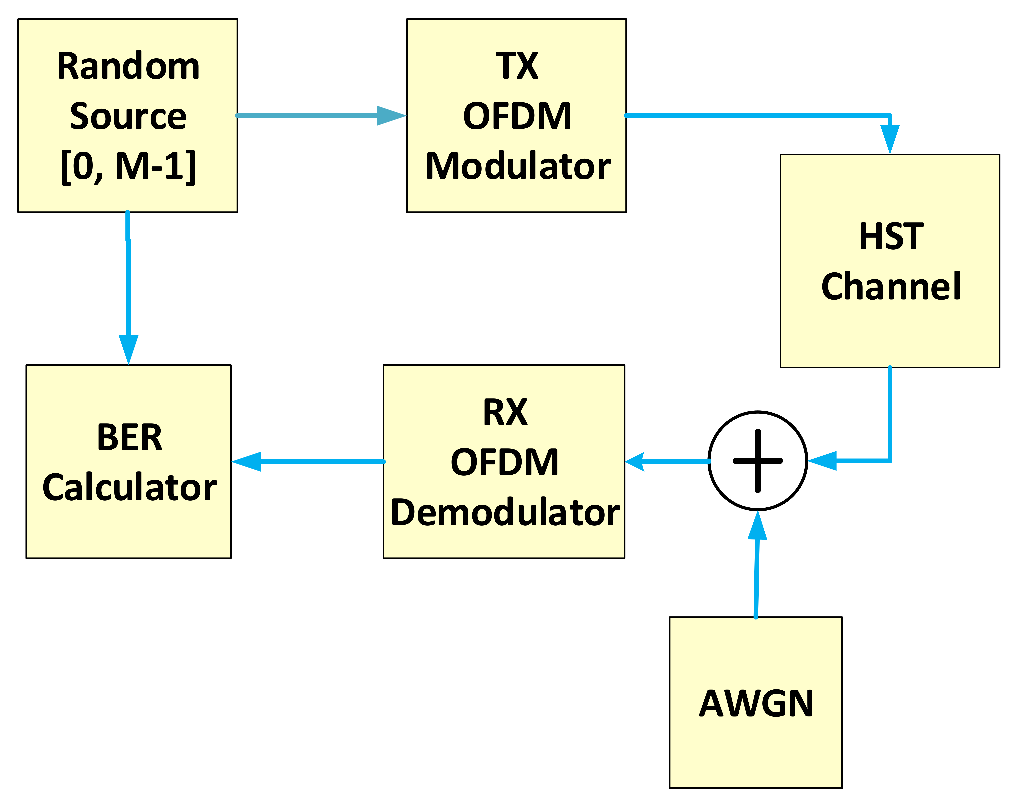
\includegraphics[width=\linewidth,keepaspectratio]{images/Gill/lte_figs/finalblock.eps} 
\caption{Block diagram of a communication system through a HST channel using QPSK, 16-QAM and 64-QAM.}
\end{figure}
The below table gives the tunnel parameters which we used in the thesis for MATLAB simulaton.

\begin{table*}[t!]
\centering
\caption{Tunnel and Tx/Rx Characteristics}
\begin{tabular}{c  c  c }
   & Dimensions & Simulation Parameters\\\hline
Tunnel & Width = 8.6 m, Height = 7.3 m & $\varepsilon_r = 5$, $\sigma = 0.1~\textrm{Sm}^{-1}$\\\hline
Leaky Feeder Cable (Tx) & Height = 6.1 m & $f_c$ (GHz) = 2, 3, 5\\\hline
Train (Rx) & Height = 4.2 m &  v (km/h) = 300, 400, 500\\
\hline
\end{tabular}
\label{tablelter}
\end{table*}


\subsection{HST Channel Model}

\begin{figure}[!ht]
\label{subblock}
\centering
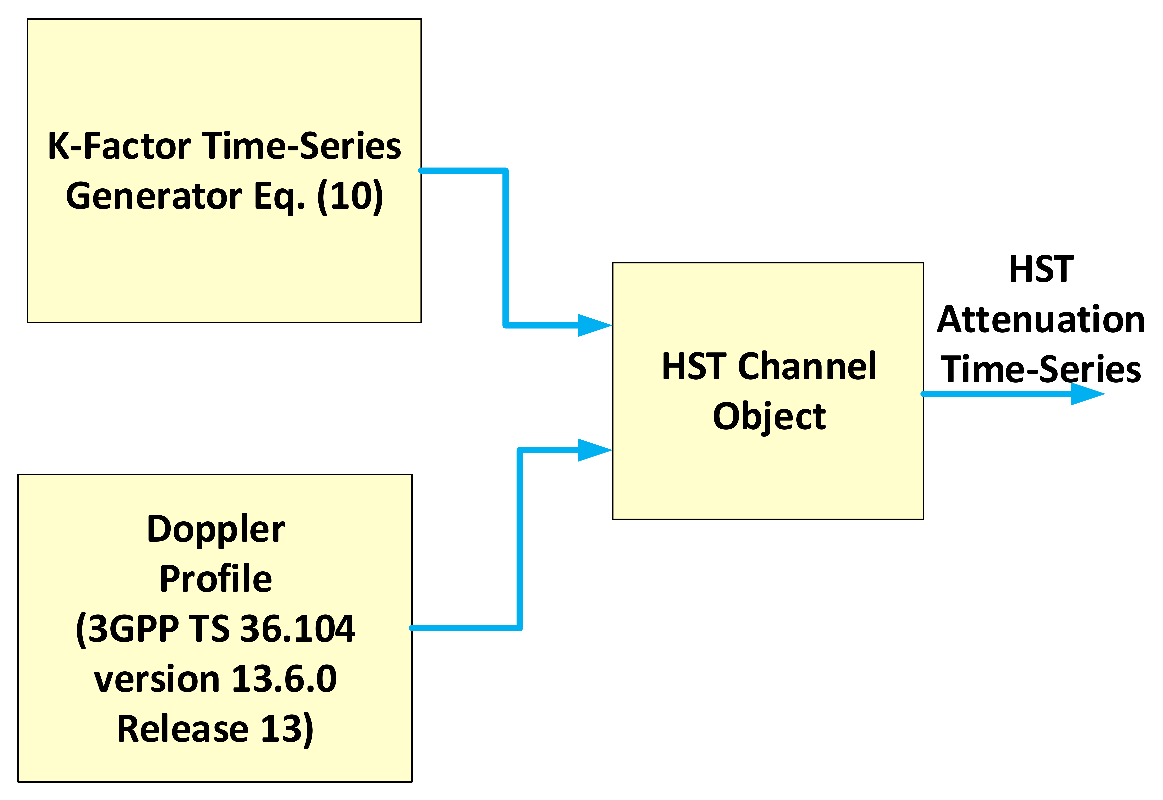
\includegraphics[width=\linewidth,keepaspectratio]{images/Gill/lte_figs/subblock.eps} 
\caption{HST channel model consisting of time-series K-factor and Doppler shift caused due to velocity of the train.}
\end{figure}



\subsection{LTE-R OFDMA}

\begin{figure}[!ht]
\label{lteofdma}
\centering
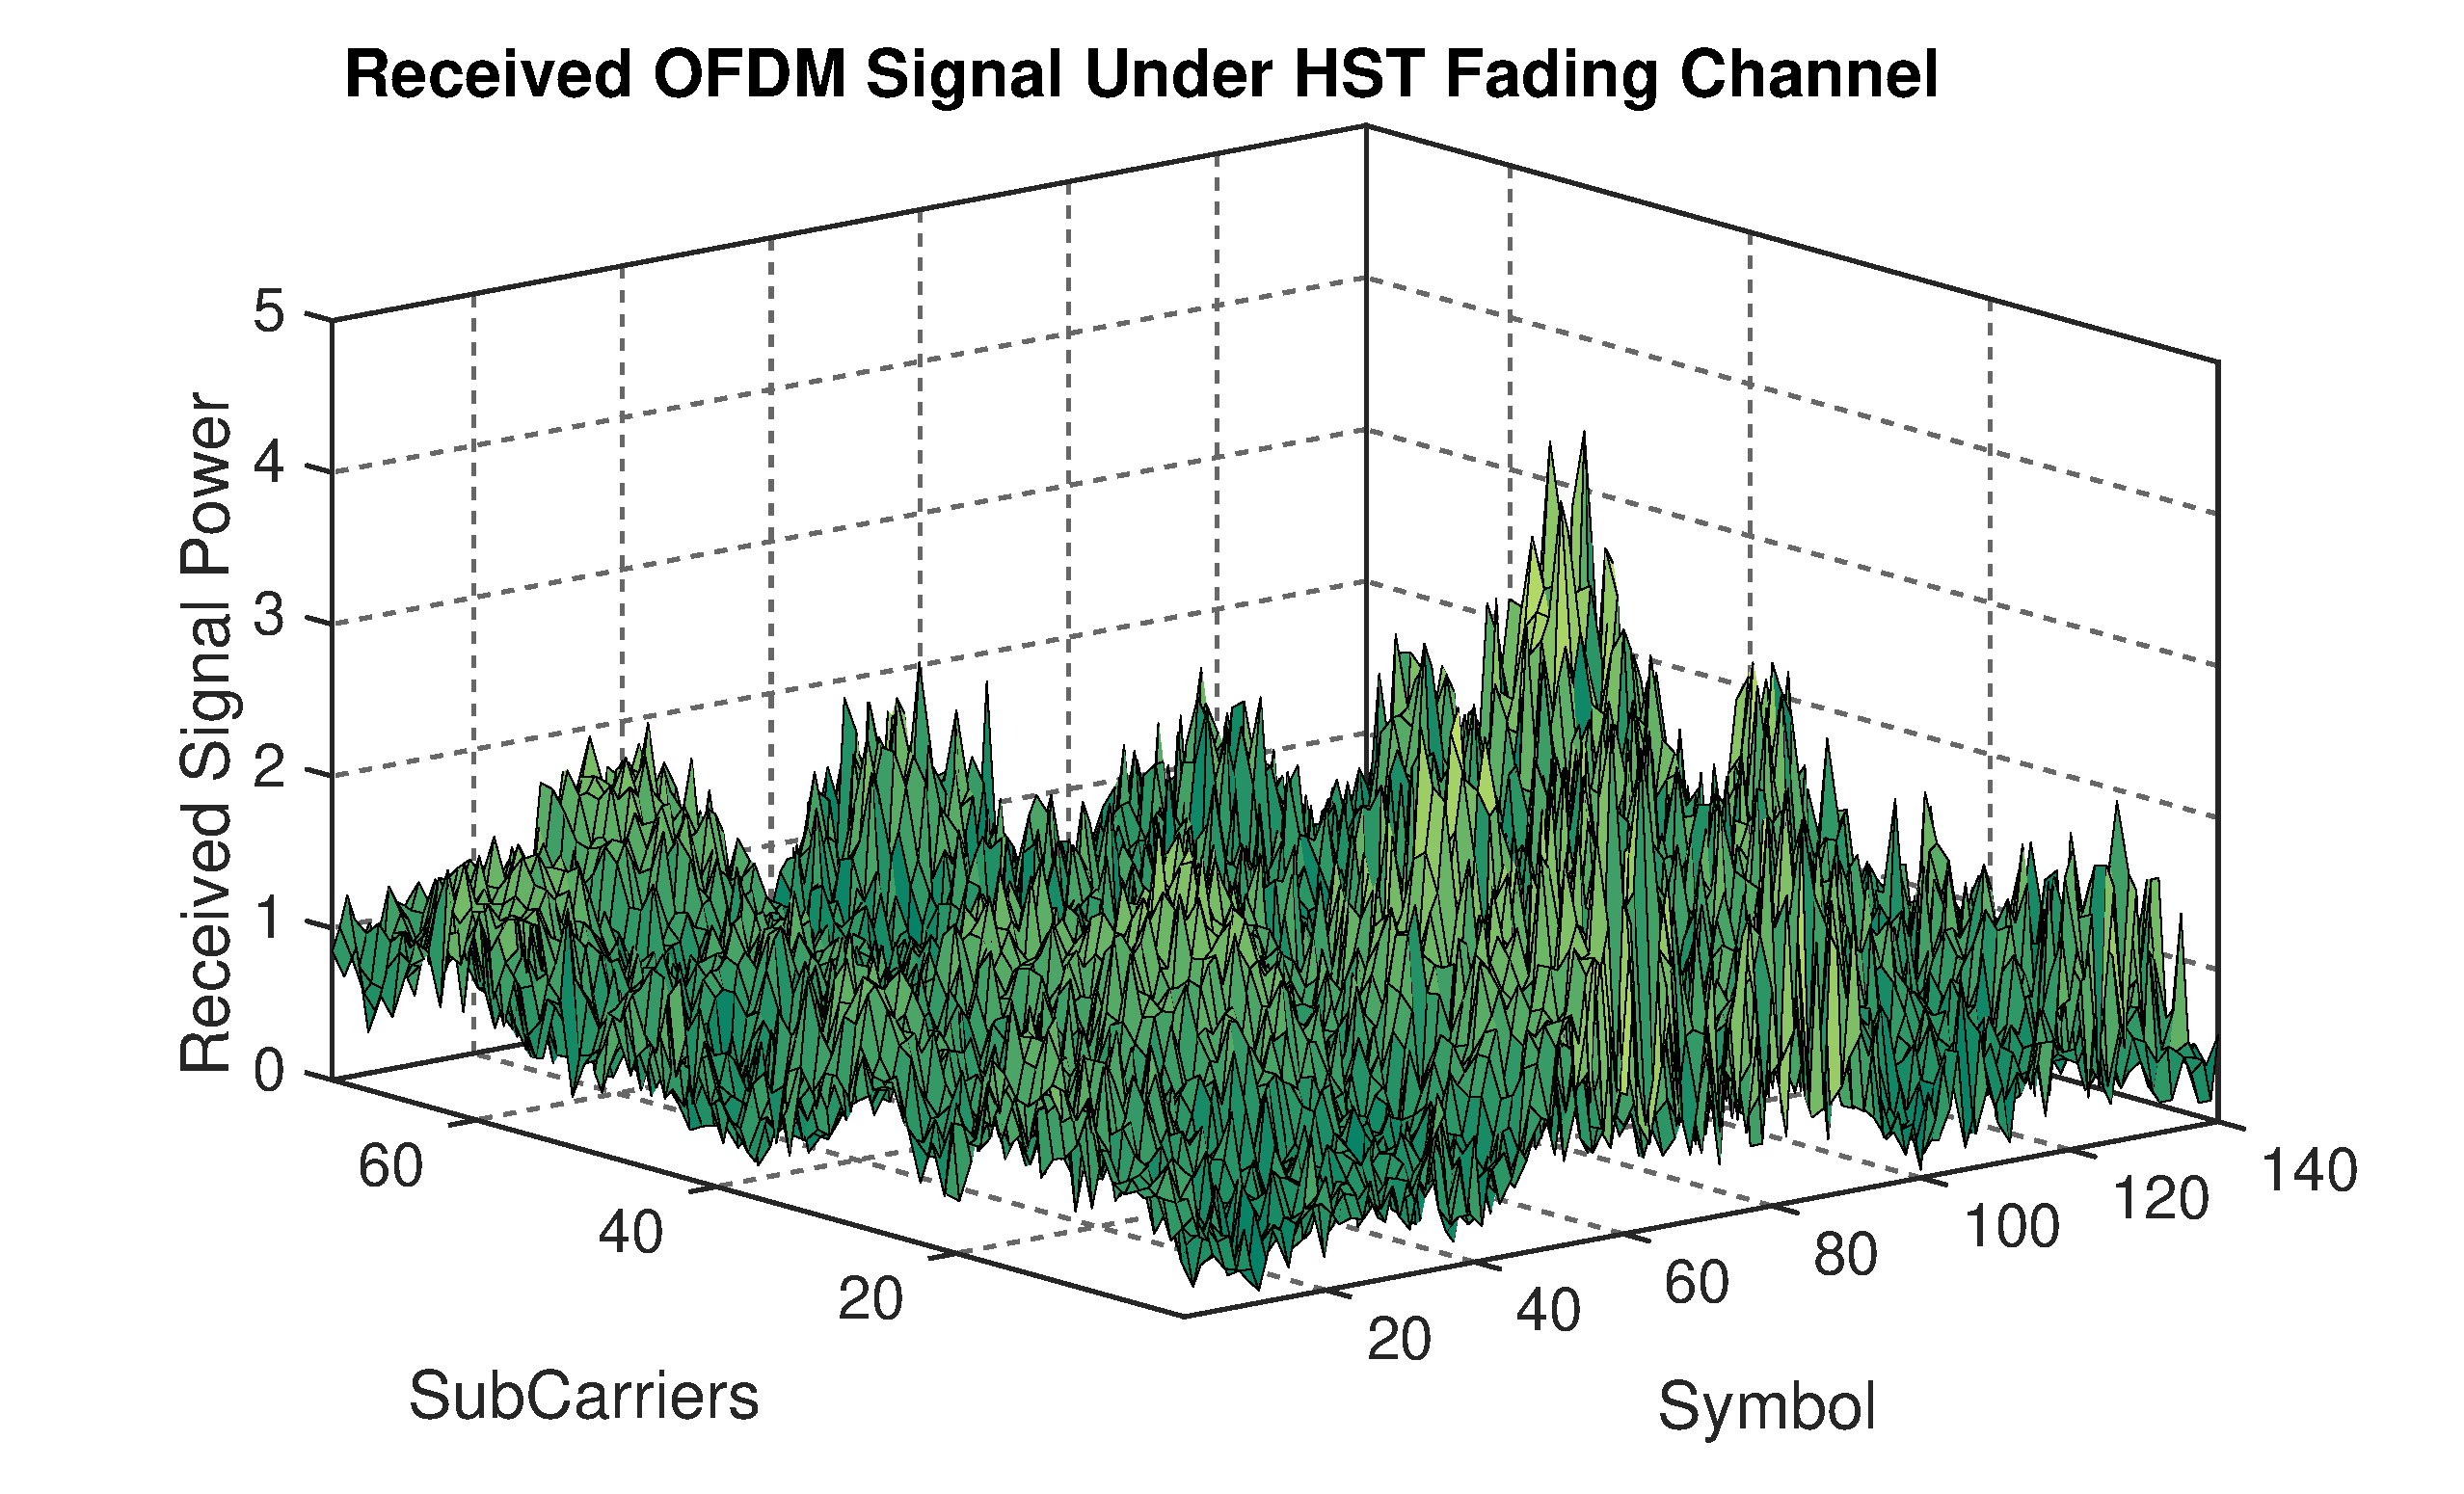
\includegraphics[width=\linewidth,keepaspectratio]{images/Gill/lte_figs/receivedsignal.eps} 
\caption{Received LTE-R OFDM signal under HST Ricean Fading Environment. }
\end{figure}





\section{Analysis}

\section{Summary}
This chapter discussed the implementation fall-backs and successes of the BLISS system.  The entire AS\textsuperscript{6} system was outlined and scrutinized for feasibility and operational performance.  Spectral Subtraction and Signal Separation were transitioned from original research goals to more manageable problems, with simplified solutions.  Overall it can be said that optimality and technical complexity were sacrificed in the end for realizability.  Many directions needed to be changed, especially in the Signal Separation block, and constraints needed to be tightened on the Spectral Subtraction block.  Although AntSS couldn't be realized a solid foundation exists for future work.\\ 




